\section{Aufbau}

Der Aufbau besteht aus einem dünnen, von der Decke hängenden Stahlseil, an dessen Ende eine Metallkugel befestigt ist. Die Messung wird erneut mit Hilfe einer Lichtschranke duchgeführt.

\section{Bestimmung der Fallbeschleunigung}

\section{Mathematische Grundlagen}

Um die Fallbeschleunigung g der Erde mit Hilfe eines Pendels zu bestimmen, muss man zunächst eine Entscheidung darüber fällen, ob man mit dem Modell eines mathematischen oder eines physikalischen Pendels modellieren sollte.
In diesem Versuch wird das physikalische Pendel verwendet, da die Versuchbedinungen nicht idealisiert waren und das mathematische Modell daher zu ungenau wäre.

Da das Pendel für diesen Versuch um kleinen Winkel von ca. 5° augelenkt wurde, wird auf die Kleinwinkelannäherung des physikalischen Pendels zurückgegriffen

\begin{align}
	\label{eq:physikalisches-pendel}
	T = 2 \pi \sqrt{\frac{\theta}{m g d}}  \implies T^2 = 4 \pi^2 \frac{\theta}{m g d} \implies g = \frac{4 \pi^2 \theta}{m d T^2} .
\end{align}

Das Trägheitsmoment $\theta$ des Pendels setzt sich aus dem Trägheitsmoment der Kugel und dem Trägheitsmoment nach dem Satz von Steiner zusammen.
Da man die Kugel als Kugelkreisel ansehen kann, ergibt sich vereinfacht

\begin{align}
	\theta = \theta_\text{Kugel} + \theta_\text{Steiner} = \frac{2}{5} m r^2 + m d^2 .
\end{align}

Da das Pendel für diesen Versuch um kleinen Winkel von ca. 5° augelenkt wurde, wird auf die Kleinwinkelannäherung des physikalischen Pendels zurückgegriffen:

Nach einsetzen in \ref{eq:physikalisches-pendel} ergibt sich

\begin{align}
	\label{eq:ortsfaktor}
	g = \frac{4 \pi^2 m (\frac{2}{5} r^2 + d^2)}{m d T^2} = 4 \pi^2 \frac{\frac{2}{5} r^2 + d^2}{d T^2}
\end{align} .

Die Periodendauer $T$ errechnet sich aus den Messwerten des Versuchs, die Länge $d$ des Pendelfadens ist als 2,355m gegeben und mit einem systematischen Fehler von 3mm behaftet.

Zuletzt wird der Radius der Kugel benötigt. Um diesen zu ermitteln, wurde der Durchmesser $D$ der Kugel dreimal mit einem Messschieber gemessen und über die Werte gemittelt.

\section{Auswertung}

Die Berechnung der Periodendauer wird durch Regression ausgeführt.

\begin{figure}[h!]
    \centering
    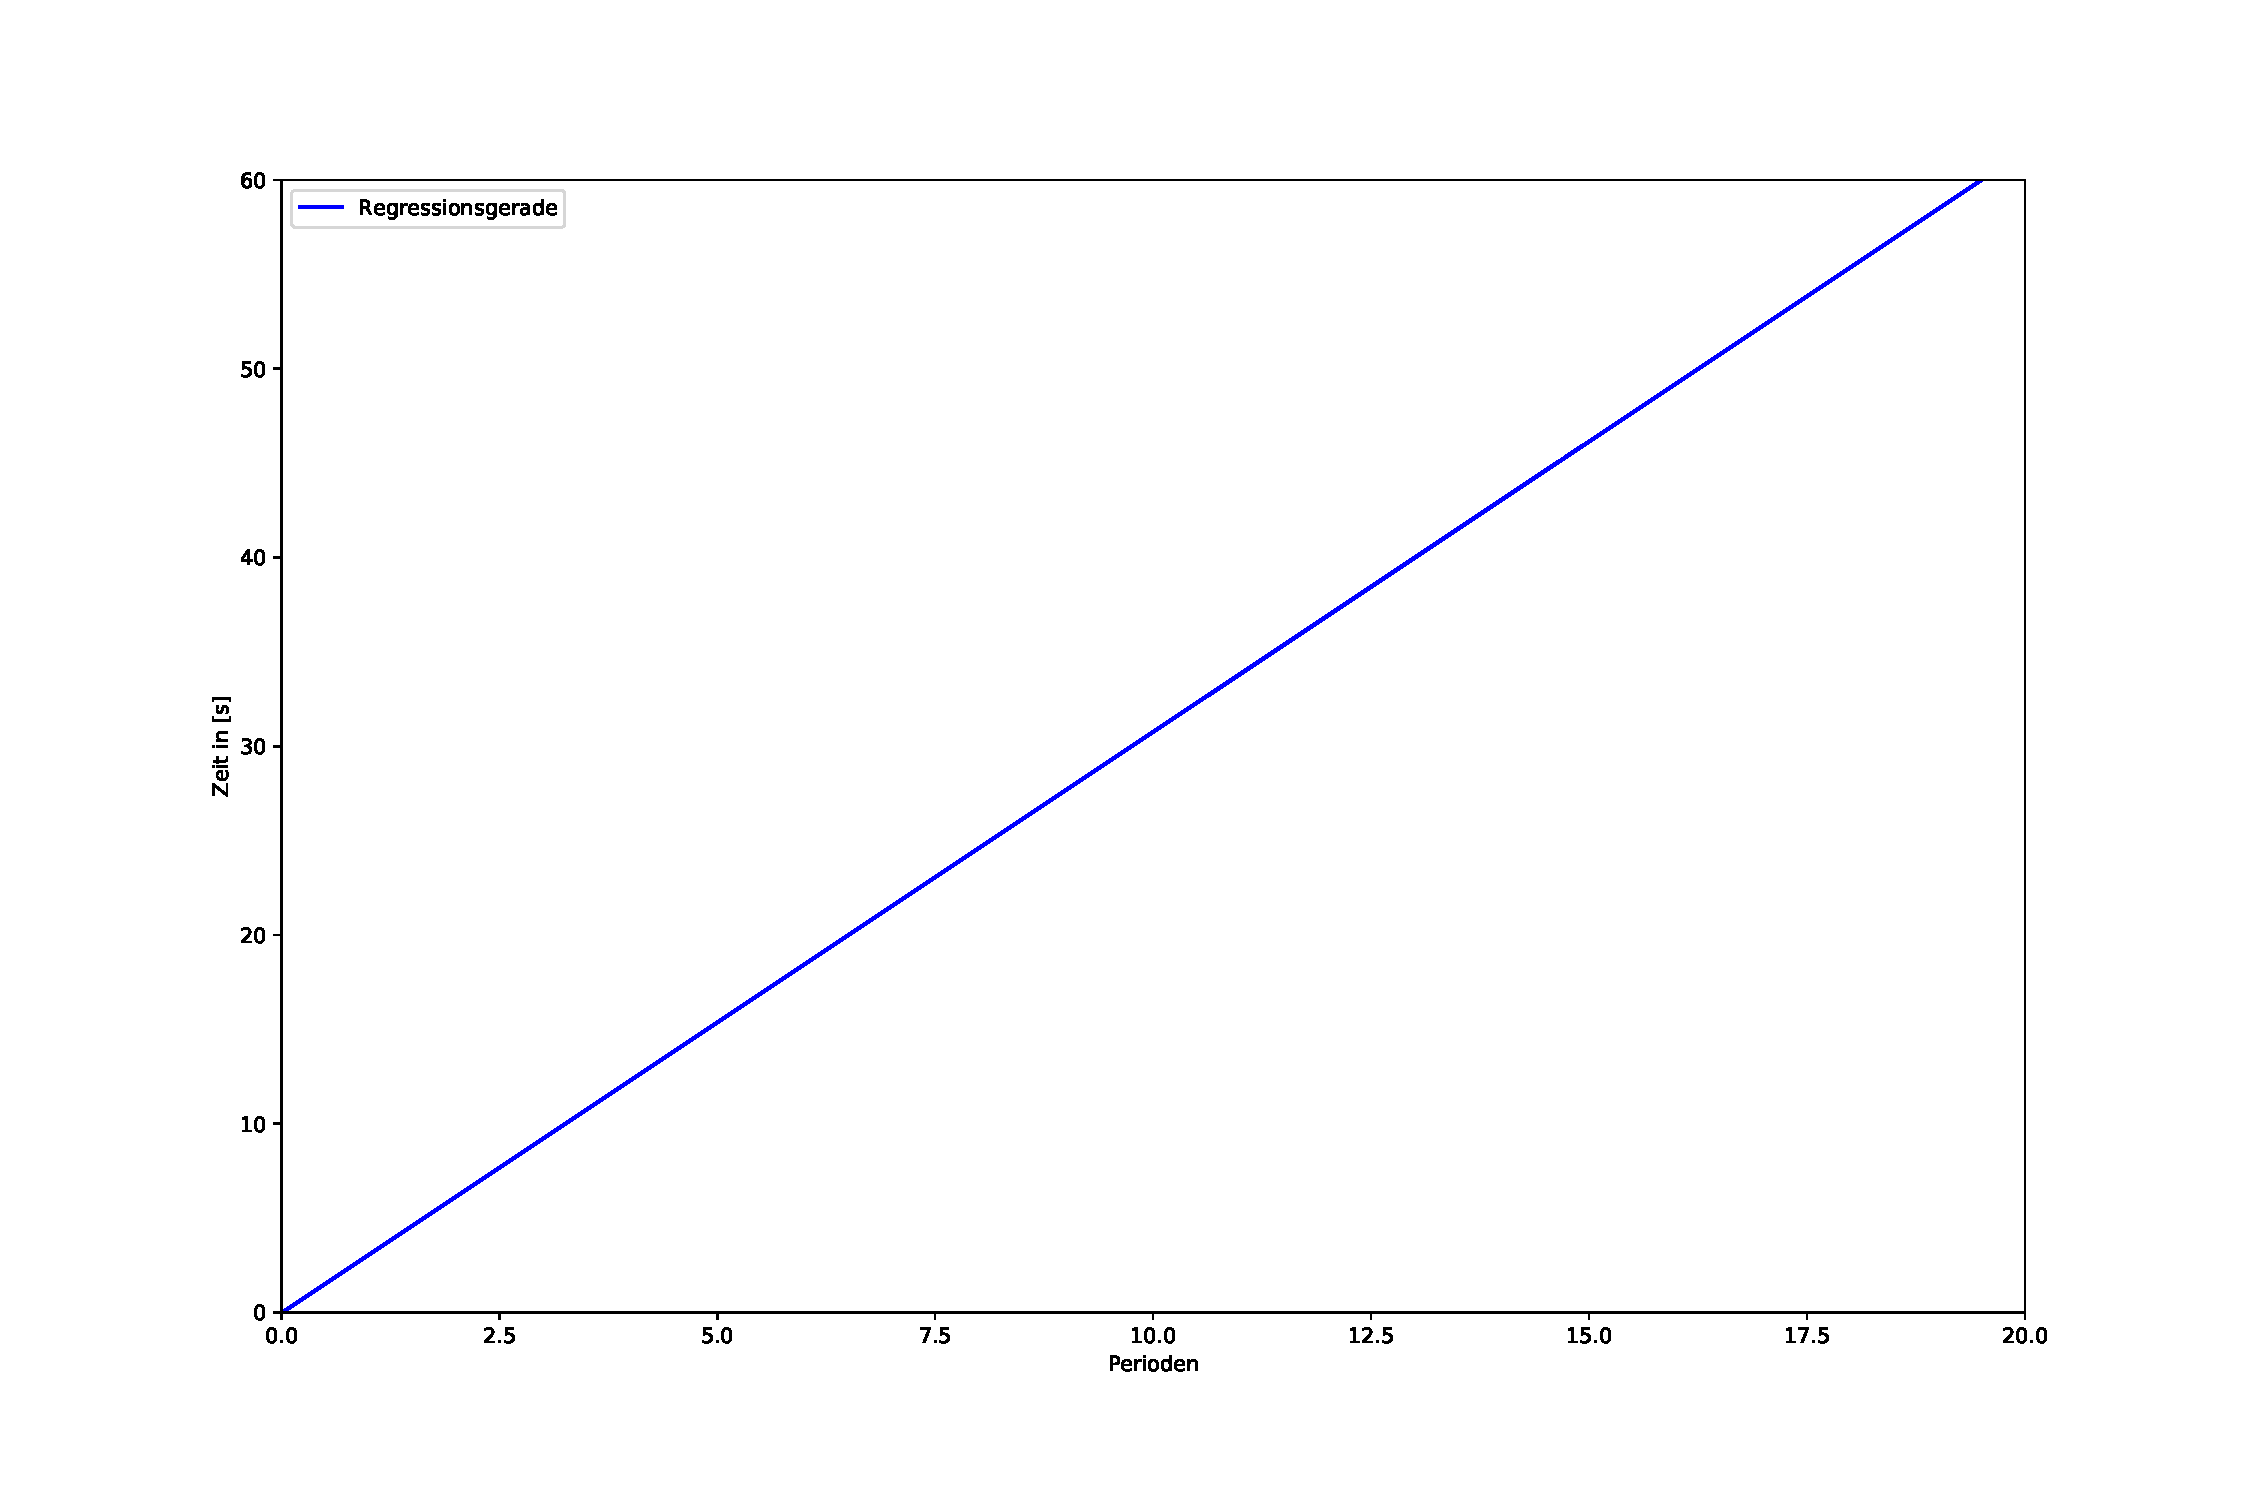
\includegraphics[scale=0.5]{./Pendel/Protokoll/fig/Fadenpendel_Regression.pdf
    }
    \caption{Regression der Messwerte}
    \label{fig:Venturi}
\end{figure}

Aus der Regression ergibt sich für $T$ ein Wert von $3.079s$, mit einer statistischen Fehlerbehaftung von $0,000018s$.

Der Radius der Kugel errechnet sich wie folgt:

$D_M = \frac{D_1 + D_2 + D_3}{3}$
$r = \frac{D_M}{2}$

Der Durchmesser der Kugel wurde zu $0,060m$, $0,059m$ und $0,060m$ gemessen.
Aufgrund der Ungenauigkeit des Messchiebers, werden die $D_i$ mit einem systematischen Fehler von $0,005m$ behaftet, wozu noch eine Standardabweichung zu $0,0006$m als statistischer Fehler hinzukommt.

Es ergibt sich demnach $r = 0,03m$ mit einem statistischen Fehler von $0,0003m$ und einem einem systematischen Fehler von $0,0025m$.

Nach \ref{eq:ortsfaktor} ergibt sich

$g = 9,8075\frac{m}{s^2}$

Zur Fehlerrechnung wird Gaußsche Fehlerfortpflanzung verwendet. Dies ist möglich, da man aufgrund der ungenauen Messmethode den Zusammenhang von r und d vernachlässigen kann und somit alle Fehler unkorreliert sind.



\section{Abhängigkeit der Schwingungsdauer von der Schwingungsweite}